\documentclass{chi-ext}
% Please be sure that you have the dependencies (i.e., additional LaTeX packages) to compile this example.
% See http://personales.upv.es/luileito/chiext/

%% EXAMPLE BEGIN -- HOW TO OVERRIDE THE DEFAULT COPYRIGHT STRIP -- (July 22, 2013 - Paul Baumann)
% \copyrightinfo{Permission to make digital or hard copies of all or part of this work for personal or classroom use is granted without fee provided that copies are not made or distributed for profit or commercial advantage and that copies bear this notice and the full citation on the first page. Copyrights for components of this work owned by others than ACM must be honored. Abstracting with credit is permitted. To copy otherwise, or republish, to post on servers or to redistribute to lists, requires prior specific permission and/or a fee. Request permissions from permissions@acm.org. \\
% {\emph{IHM14}}, 28-31 Octobre, 2014, Lille, France. \\
% Copyright \copyright~2014 ACM ISBN/14/04...\$15.00. \\
% DOI string from ACM form confirmation}
%% EXAMPLE END -- HOW TO OVERRIDE THE DEFAULT COPYRIGHT STRIP -- (July 22, 2013 - Paul Baumann)

\title{Test of Adaptable User Interfaces}

\numberofauthors{4}
% Notice how author names are alternately typesetted to appear ordered in 2-column format;
% i.e., the first 4 autors on the first column and the other 4 auhors on the second column.
% Actually, it's up to you to strictly adhere to this author notation.
\author{
  \alignauthor{
  	\textbf{Nelson}\\
  	\affaddr{AuthorCo, Inc.}\\
  	\affaddr{123 Author Ave.}\\
  	\affaddr{Authortown, PA 54321 USA}\\
  	\email{author1@anotherco.com}
  }\alignauthor{
  	\textbf{Julien}\\
  	\affaddr{AuthorCo, Inc.}\\
  	\affaddr{123 Author Ave.}\\
  	\affaddr{Authortown, PA 54321 USA}\\
  	\email{author5@anotherco.com}
  }
  \vfil
  \alignauthor{
  	\textbf{Lydie}\\
  	\affaddr{AuthorCo, Inc.}\\
  	\affaddr{123 Author Ave.}\\
  	\affaddr{Authortown, PA 54321 USA}\\
  	\email{author2@anotherco.com}
  }\alignauthor{
  	\textbf{Sophie}\\
  	\affaddr{AuthorCo, Inc.}\\
  	\affaddr{123 Author Ave.}\\
  	\affaddr{Authortown, PA 54321 USA}\\
  	\email{author6@anotherco.com}
  }
}

% Paper metadata (use plain text, for PDF inclusion and later re-using, if desired)
\def\plaintitle{Test of Adaptable User Interfaces}
\def\plainauthor{Nelson Mariano Leite Neto}
\def\plainkeywords{Guides, instructions, author's kit, conference publications}
\def\plaingeneralterms{Documentation, Standardization}

\hypersetup{
  % Your metadata go here
  pdftitle={\plaintitle},
  pdfauthor={\plainauthor},  
  pdfkeywords={\plainkeywords},
  pdfsubject={\plaingeneralterms},
  % Quick access to color overriding:
  %citecolor=black,
  %linkcolor=black,
  %menucolor=black,
  %urlcolor=black,
}

\usepackage{graphicx}   % for EPS use the graphics package instead
\usepackage{balance}    % useful for balancing the last columns
\usepackage{bibspacing} % save vertical space in references
%\usepackage{hyperref}
%\hypersetup{colorlinks=false}

%\widowpenalty=10000
%\clubpenalty=10000

\begin{document}

\maketitle

\begin{abstract}
TODO - Lorem ipsum sed ut perspiciatis unde omnis iste natus error sit voluptatem accusantium doloremque laudantium, totam rem aperiam, eaque ipsa quae ab illo inventore veritatis et quasi architecto beatae vitae dicta sunt explicabo. Nemo enim ipsam voluptatem quia voluptas sit aspernatur aut odit aut fugit, sed quia consequuntur magni dolores eos qui ratione voluptatem sequi nesciunt. Neque porro quisquam est, qui dolorem ipsum quia dolor sit amet, consectetur, adipisci velit, sed quia non numquam eius modi tempora incidunt ut labore et dolore magnam aliquam quaerat voluptatem.
\end{abstract}

\keywords{\plainkeywords}
\textcolor{red}{Champs requis dans la version finale}

\category{H.5.m}{Information interfaces and presentation (e.g., HCI)}{Miscellaneous}. 
%See \cite{ACMCCS} 
Voir : \url{http://www.acm.org/about/class/1998/} 
pour une description du ACM Classification system.
\textcolor{red}{Champs requis dans la version finale}

\terms{\plaingeneralterms}
\textcolor{red}{Champs requis dans la version finale}


% =============================================================================
\section{Introduction}
% =============================================================================
TODO

% =============================================================================
\section{Related Work}
% =============================================================================
TODO

% =============================================================================
\section{Case Study}
% =============================================================================

\marginpar{
\begin{figure}
  \begin{center}
  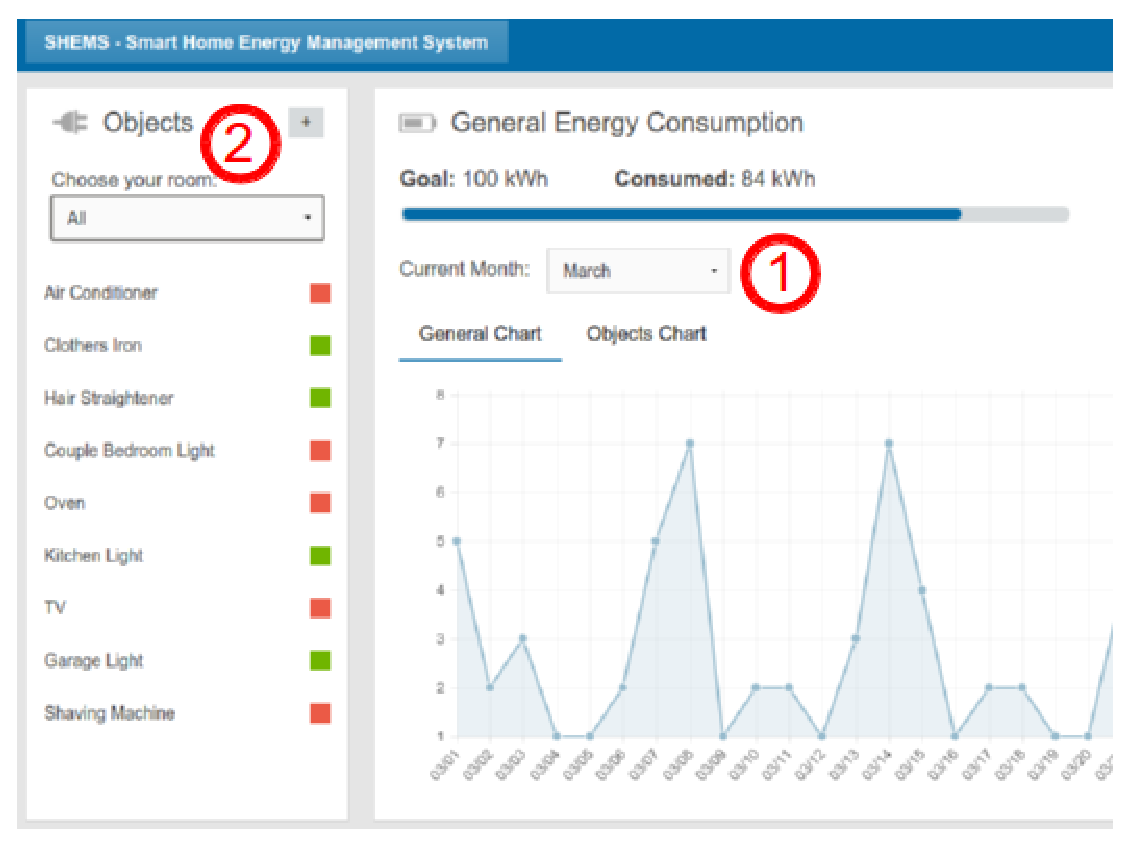
\includegraphics[width=\marginparwidth]{images/web0_goal-filter.eps}
  \caption{Une figure dans la marge.}
  \label{fig:marginparsample}
  \end{center}  
\end{figure}

\begin{figure}
  \begin{center}
  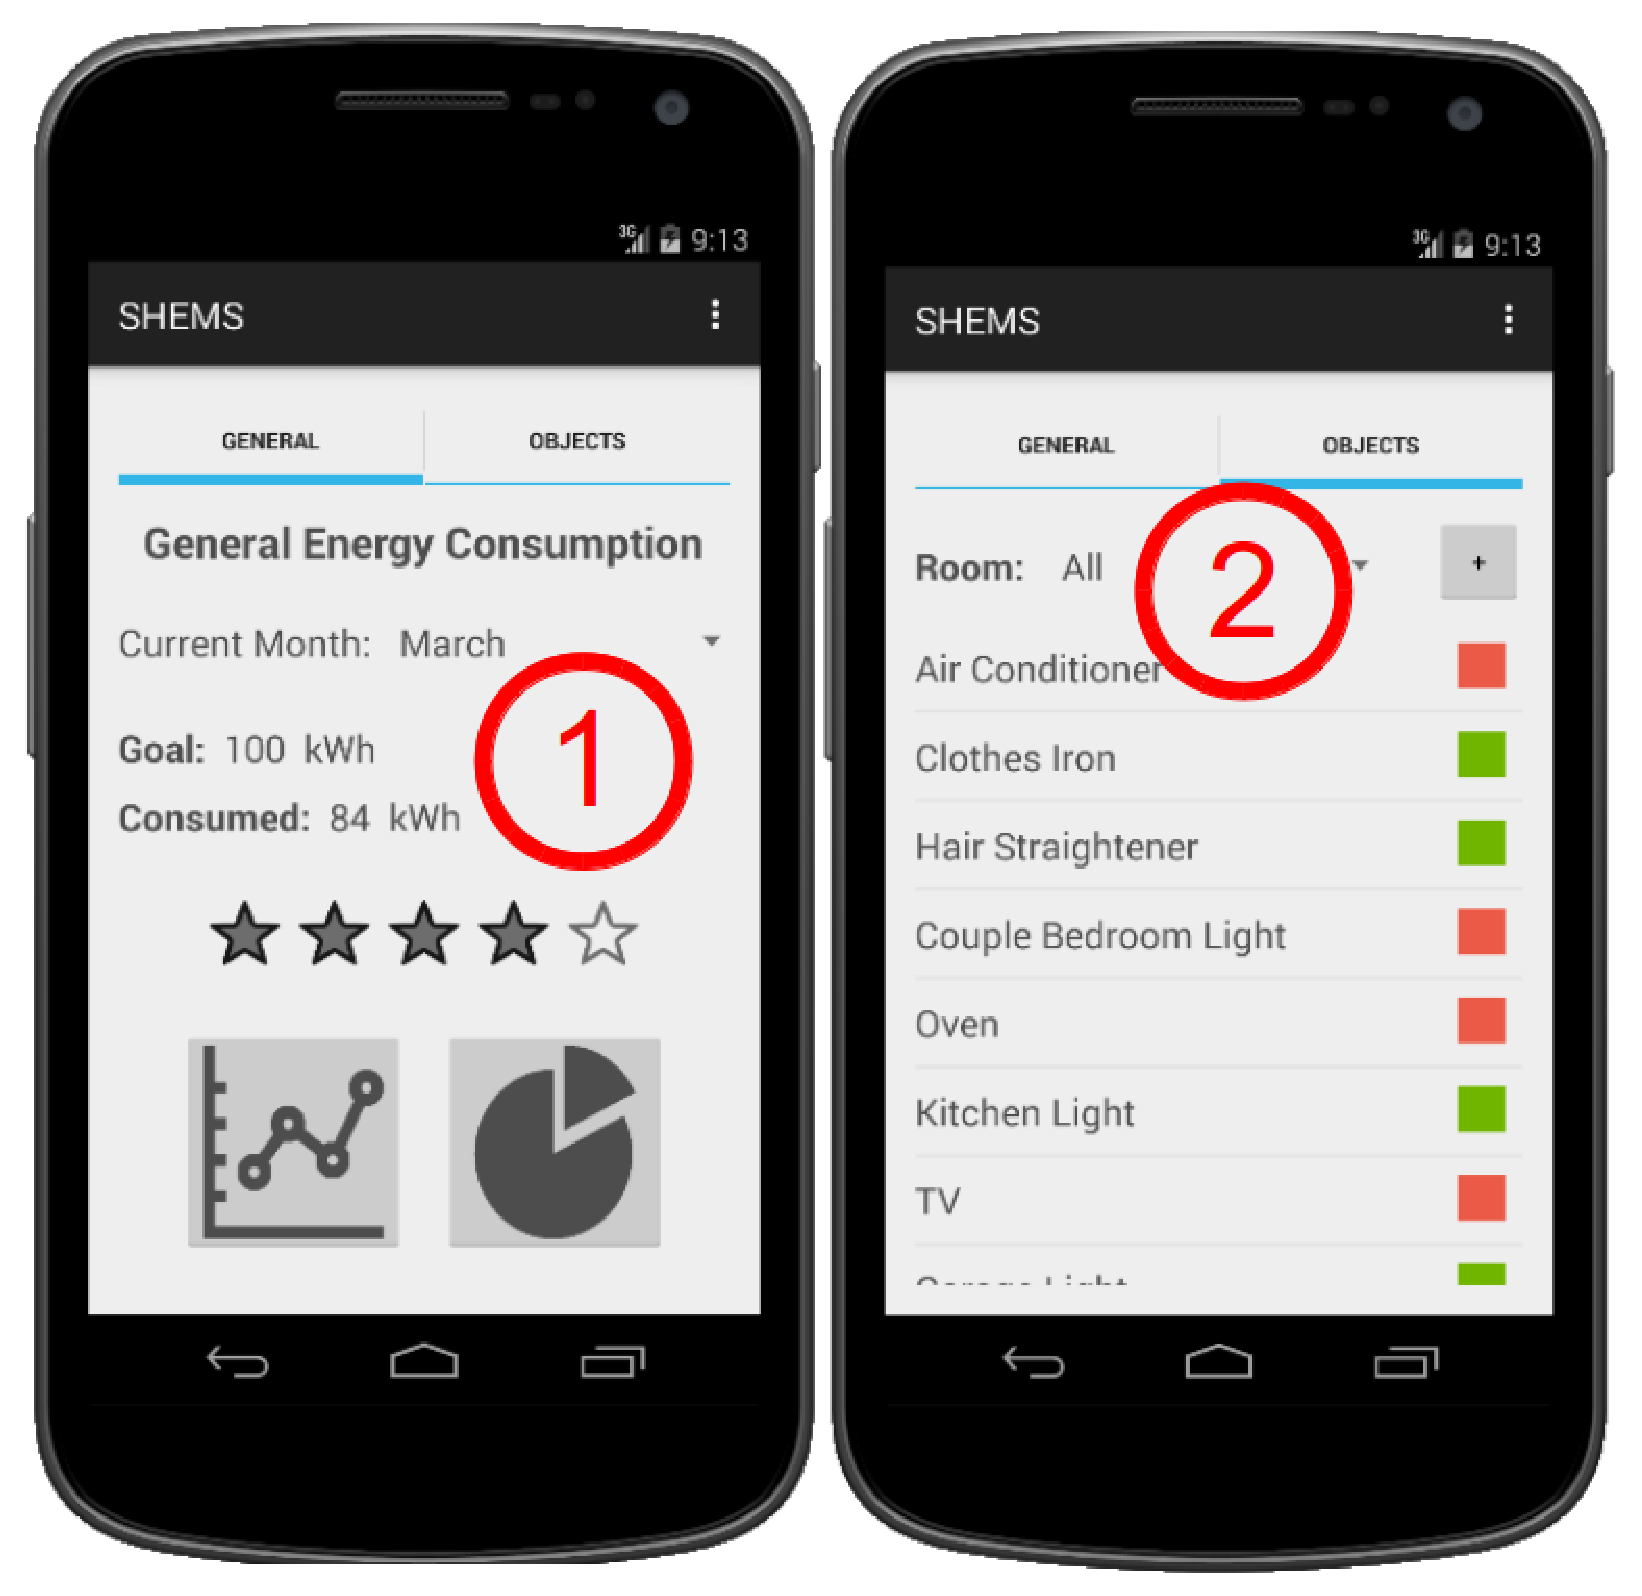
\includegraphics[width=\marginparwidth]{images/mobile_goal-filter.eps}
  \caption{Une figure dans la marge.}
  \label{fig:marginparsample}
  \end{center}  
\end{figure}
}

The case study used in this work is a prototype for a smart home energy management system. This decision is based on the fact that it is a modern concept, little explored in the domain of this research and whose UIs can be adapted to several contexts. A smart home may be defined as a well-designed structure with sufficient access to assets, communication, controls, data, and information technologies for enhancing the occupants' quality of life through comfort, convenience, reduced costs and increased connectivity~\cite{smart-home-harper}. A smart home energy management system is an energy management system applied to smart homes. It allows users to control and monitor the energy consumption in a residence from different devices. 

It is a prototype because we have developed only the UIs of the system for four versions, three for web environment and one as a mobile application. The data of the system are predetermined. All versions have the same features, except for two web versions that have an additional feature. The differences between the versions are visual. In the case of the mobile application, the UI is adapted to a mobile device, which contains a smaller screen and its own platform for UI development. In the case of the web versions, the UIs have also been developed to this context, using web UI technologies. But the differences between the three web versions are changes in the navigation and UI components. In this paper, we focus on the following features of the prototype:

\begin{enumerate}

\item \textbf{Goal}: the user can check information about the general energy consumption per month. Having access to the goal and consumption in kWh for the chosen month. 

\item \textbf{Filter}: the user has access to a list of all his or her objects in the house, having the possibility to filter this list per room. An object means any component that can be controlled and whose energy consumption can be registered, such as lights and electronic devices.

\item \textbf{Comparator}: the user can choose two objects and compare, side by side, their energy consumption charts. This feature is present in only two of the web versions.

\end{enumerate} 

\begin{figure}
  \centering
  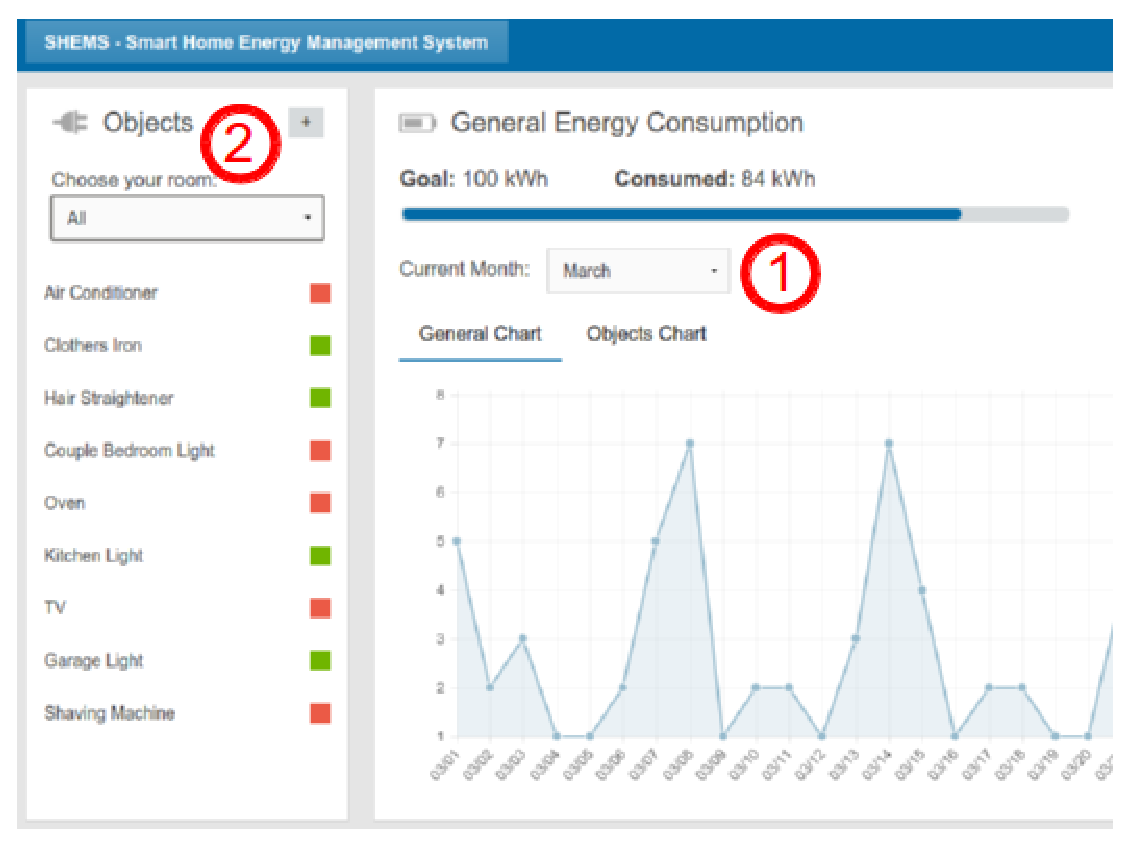
\includegraphics[width=\linewidth]{images/web0_goal-filter.eps}
  \caption{Ajoutez une légende en dessous de chaque image.}
  \label{fig:sample}
\end{figure}

\begin{figure}
  \centering
  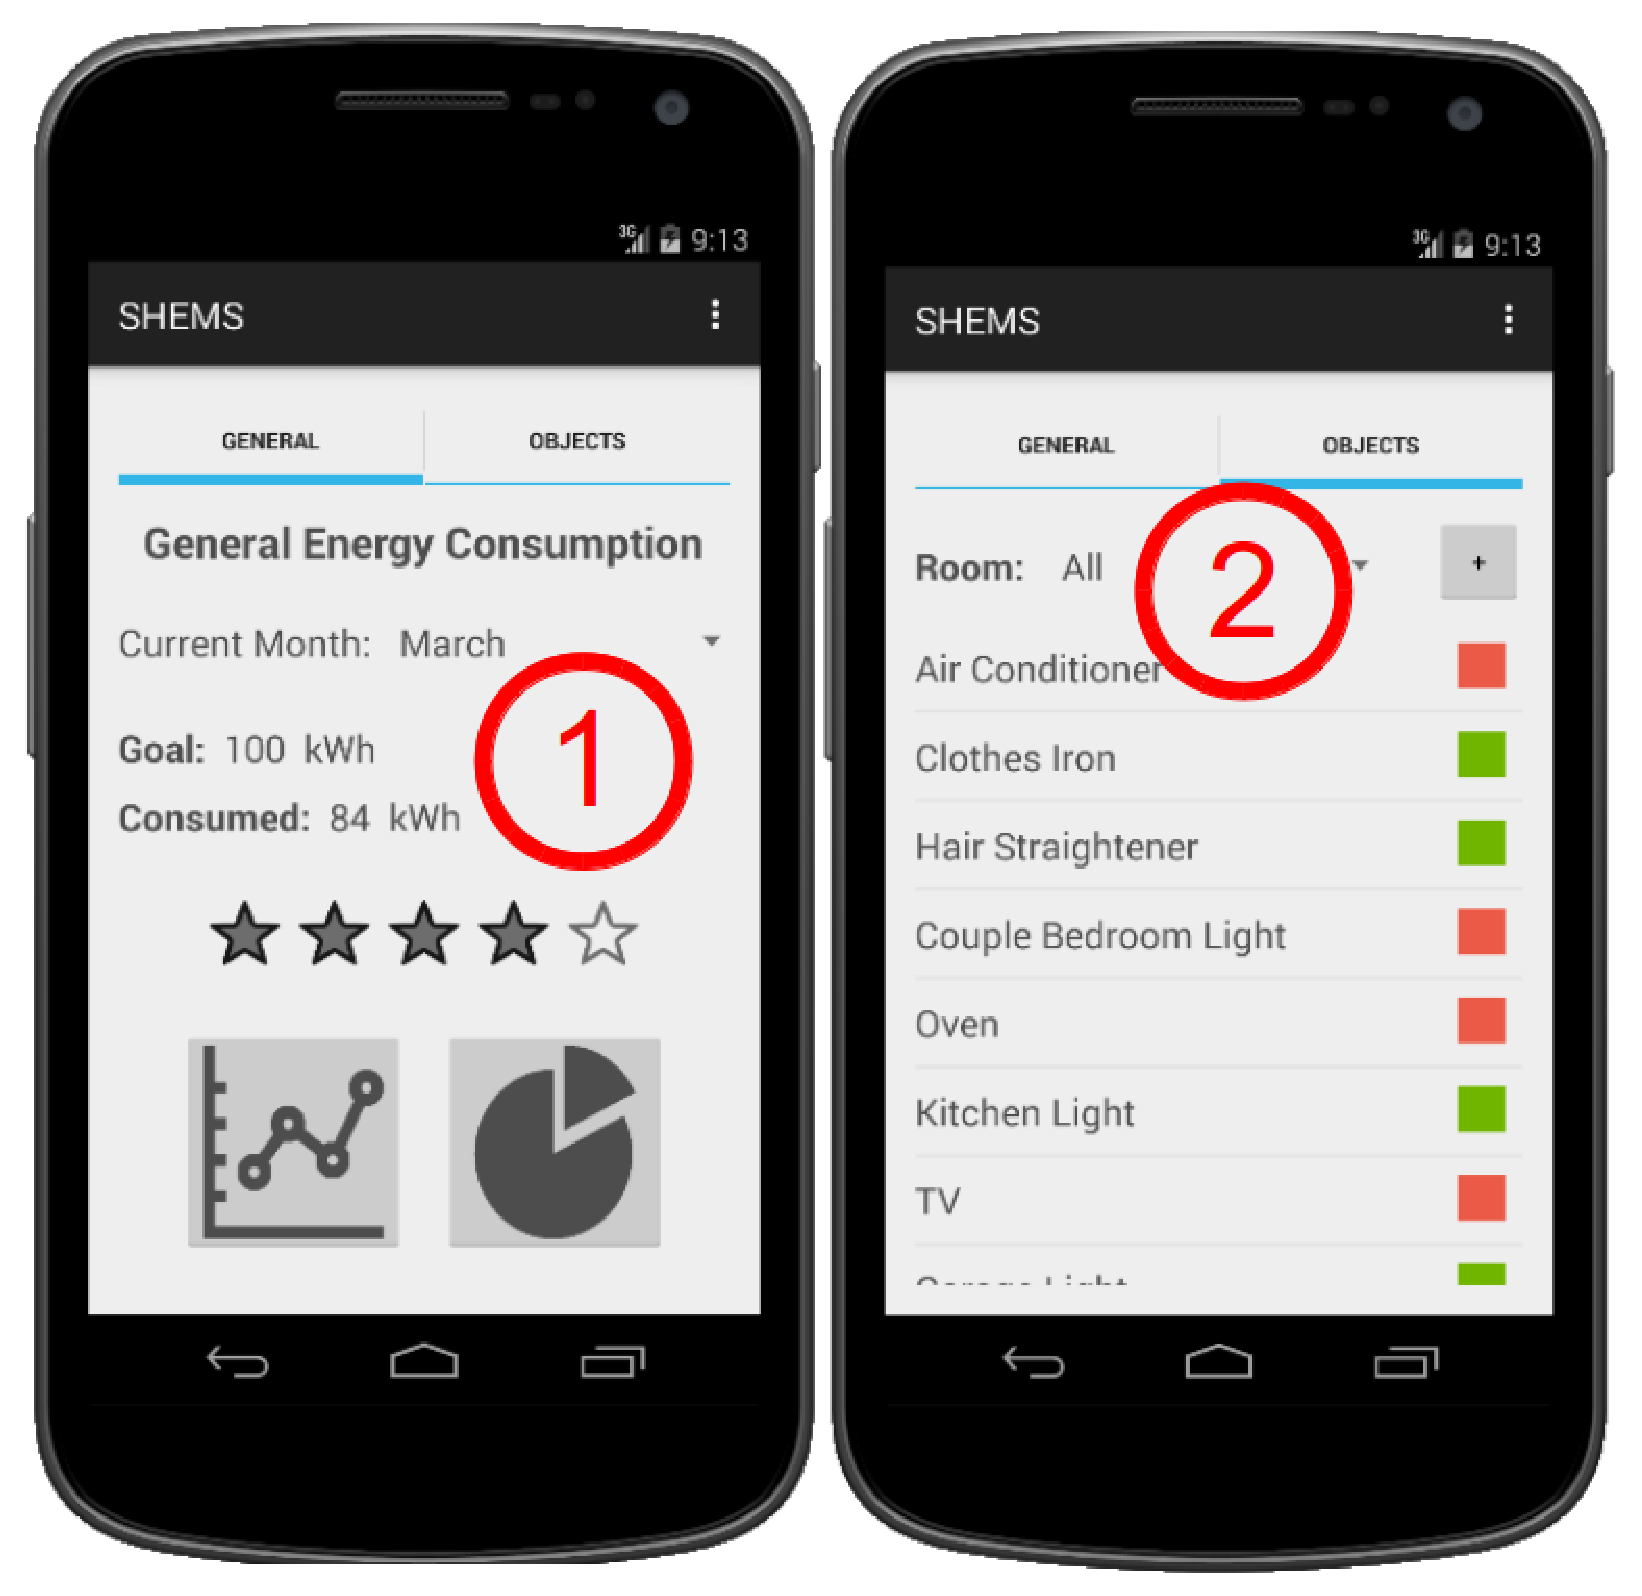
\includegraphics[width=\linewidth]{images/mobile_goal-filter.eps}
  \caption{Ajoutez une légende en dessous de chaque image.}
  \label{fig:sample}
\end{figure}

% =============================================================================
\section{Approach: generating test scripts for UI testing from abstract descriptions}
% =========================================
\subsection{Principle}
TODO

\subsection{Principles put into Practice}
TODO

\subsection{Discussion and Analysis}
TODO

% =============================================================================
\section{Conclusions and Perspectives}
% =============================================================================
TODO

\balance
\bibliographystyle{acm-sigchi}
\bibliography{ref}

\end{document}